%% abtex2-modelo-trabalho-academico.tex, v-1.9.2 laurocesar
%% Copyright 2012-2014 by abnTeX2 group at http://abntex2.googlecode.com/ 
%%
%% This work may be distributed and/or modified under the
%% conditions of the LaTeX Project Public License, either version 1.3
%% of this license or (at your option) any later version.
%% The latest version of this license is in
%%   http://www.latex-project.org/lppl.txt
%% and version 1.3 or later is part of all distributions of LaTeX
%% version 2005/12/01 or later.
%%
%% This work has the LPPL maintenance status `maintained'.
%% 
%% The Current Maintainer of this work is the abnTeX2 team, led
%% by Lauro César Araujo. Further information are available on 
%% http://abntex2.googlecode.com/
%%
%% This work consists of the files abntex2-modelo-trabalho-academico.tex,
%% abntex2-modelo-include-comandos and abntex2-modelo-references.bib
%%

% ------------------------------------------------------------------------
% ------------------------------------------------------------------------
% abnTeX2: Modelo de Trabalho Academico (tese de doutorado, dissertacao de
% mestrado e trabalhos monograficos em geral) em conformidade com 
% ABNT NBR 14724:2011: Informacao e documentacao - Trabalhos academicos -
% Apresentacao
% ------------------------------------------------------------------------
% ------------------------------------------------------------------------

%-------------------------------------------------------------------------
% Modelo adaptado especificamente para o contexto do PPgSI-EACH-USP por 
% Marcelo Fantinato, com auxílio dos Professores Norton T. Roman, Helton
% H. Bíscaro e Sarajane M. Peres, em 2015, com muitos agradecimentos aos 
% criadores da classe e do modelo base.
%
% 20/06/2017: inclusão de "lista de quadros" com base no especificado em:
% https://github.com/abntex/abntex2/wiki/HowToCriarNovoAmbienteListing,
% de autoria de "Eduardo de Santana Medeiros Alexandre".
%
%-------------------------------------------------------------------------

\documentclass[
	% -- opções da classe memoir --
	12pt,				% tamanho da fonte
	% openright,			% capítulos começam em pág ímpar (insere página vazia caso preciso)
	oneside,			% para impressão apenas no anverso (apenas frente). Oposto a twoside
	a4paper,			% tamanho do papel. 
	% -- opções da classe abntex2 --
	%chapter=TITLE,		% títulos de capítulos convertidos em letras maiúsculas
	%section=TITLE,		% títulos de seções convertidos em letras maiúsculas
	%subsection=TITLE,	% títulos de subseções convertidos em letras maiúsculas
	%subsubsection=TITLE,% títulos de subsubseções convertidos em letras maiúsculas
	% -- opções do pacote babel --
	english,			% idioma adicional para hifenização
	%french,				% idioma adicional para hifenização
	%spanish,			% idioma adicional para hifenização
	brazil				% o último idioma é o principal do documento
	]{preambles/abntex2ppgsi}

% ---
% Pacotes básicos 
% ---
% \usepackage{lmodern}			% Usa a fonte Latin Modern			
% \usepackage[T1]{fontenc}		% Selecao de codigos de fonte.
\usepackage[utf8]{inputenc}		% Codificacao do documento (conversão automática dos acentos)
\usepackage{lastpage}			% Usado pela Ficha catalográfica
\usepackage{indentfirst}		% Indenta o primeiro parágrafo de cada seção.
\usepackage{color}				% Controle das cores
\usepackage{graphicx}			% Inclusão de gráficos
\usepackage{microtype} 			% para melhorias de justificação
\usepackage{pdfpages}     %para incluir pdf
\usepackage{algorithm}			% para ilustrações do tipo algoritmo
\usepackage{mdwlist}			% para itens com espaço padrão da abnt
\usepackage[noend]{algpseudocode}			%para ilustrações do tipo algoritmo
\usepackage{pgfgantt}           % modificar a largura
\usepackage{adjustbox}
\usepackage{glossaries}
\makeglossaries

% ---
% Pacotes adicionais, usados apenas no âmbito do Modelo Canônico do abnteX2
% ---
\usepackage{lipsum}				% para geração de dummy text
% ---

% ---
% Pacotes de citações
% ---
\usepackage{hyperref}
\usepackage[brazilian,hyperpageref]{backref}	 % Paginas com as citações na bibl
\usepackage[alf,abnt-etal-list=0,abnt-etal-text=it]{abntex2cite}	% Citações padrão ABNT

% \documentclass[tikz]{standalone}
\usepackage{pgfgantt} % https://pt.overleaf.com/latex/examples/gantt-charts-with-the-pgfgantt-package/jmkwfxrnfxnw
% \title{Gantt Charts with the pgfgantt Package}
% \begin{document}

\usepackage{xcolor} % text colors https://www.overleaf.com/learn/latex/Using_colours_in_LaTeX

% --- 
% CONFIGURAÇÕES DE PACOTES
% --- 

% ---
% Configurações do pacote backref
% Usado sem a opção hyperpageref de backref
\renewcommand{\backrefpagesname}{Citado na(s) página(s):~}
% Texto padrão antes do número das páginas
\renewcommand{\backref}{}
% Define os textos da citação
\renewcommand*{\backrefalt}[4]{
	\ifcase #1 %
		Nenhuma citação no texto.%
	\or
		Citado na página #2.%
	\else
		Citado #1 vezes nas páginas #2.%
	\fi}%
% ---

% ---
% Informações de dados para CAPA e FOLHA DE ROSTO
% ---

%-------------------------------------------------------------------------
% Comentário adicional do PPgSI - Informações sobre o ``instituicao'':
%
% Não mexer. Deixar exatamente como está.
%
%-------------------------------------------------------------------------
\instituicao{
	UNIVERSIDADE DE SÃO PAULO
	\par
	ESCOLA DE ARTES, CIÊNCIAS E HUMANIDADES}

%-------------------------------------------------------------------------
% Comentário adicional do PPgSI - Informações sobre o ``título'':
%
% Em maiúscula apenas a primeira letra da sentença (do título), exceto 
% nomes próprios, geográficos, institucionais ou Programas ou Projetos ou 
% siglas, os quais podem ter letras em maiúscula também.
%
% O subtítulo do trabalho é opcional.
% Sem ponto final.
%
% Atenção: o título da Dissertação/Tese na versão corrigida não pode mudar. 
% Ele deve ser idêntico ao da versão original.
%
%-------------------------------------------------------------------------
\titulo{WotPy: Solução de Problemas e Exemplo de Uso}

%-------------------------------------------------------------------------
% Comentário adicional do PPgSI - Informações sobre o ``autor'':
%
% Todas as letras em maiúsculas.
% Nome completo.
% Sem ponto final.
%-------------------------------------------------------------------------
\autor{\uppercase{Gustavo Tsuyoshi Ariga}}

%-------------------------------------------------------------------------
% Comentário adicional do PPgSI - Informações sobre o ``local'':
%
% Não incluir o ``estado''.
% Sem ponto final.
%-------------------------------------------------------------------------
\local{São Paulo}

%-------------------------------------------------------------------------
% Comentário adicional do PPgSI - Informações sobre a ``data'':
%
% Colocar o ano do depósito (ou seja, o ano da entrega) da respectiva 
% versão, seja ela a versão original (para a defesa) seja ela a versão 
% corrigida (depois da aprovação na defesa). 
%
% Atenção: Se a versão original for depositada no final do ano e a versão 
% corrigida for entregue no ano seguinte, o ano precisa ser atualizado no 
% caso da versão corrigida. 
% Cuidado, pois o ano da ``capa externa'' também precisa ser atualizado 
% nesse caso.
%
% Não incluir o dia, nem o mês.
% Sem ponto final.
%-------------------------------------------------------------------------
\data{Julho de 2023}

%-------------------------------------------------------------------------
% Comentário adicional do PPgSI - Informações sobre o ``Orientador'':
%
% Se for uma professora, trocar por ``Profa. Dra.''
% Nome completo.
% Sem ponto final.
%-------------------------------------------------------------------------
\orientador{Prof. Dr. Fábio Nakano}

%-------------------------------------------------------------------------
% Comentário adicional do PPgSI - Informações sobre o ``Coorientador'':
%
% Opcional. Incluir apenas se houver co-orientador formal, de acordo com o 
% Regulamento do Programa.
%
% Se for uma professora, trocar por ``Profa. Dra.''
% Nome completo.
% Sem ponto final.
%-------------------------------------------------------------------------
\coorientador{Prof. Dr. José de Jesús Pérez-Alcázar}

\tipotrabalho{Relatório de Atividades}

\modalidade{\textbf{Modalidade: TCC Longo (1 ano) - individual}}

\preambulo{
%-------------------------------------------------------------------------
% Comentário adicional do PPgSI - Informações sobre o texto ``Versão 
% original'':
%
% Não usar para Qualificação.
% Não usar para versão corrigida de Dissertação/Tese.
%
%-------------------------------------------------------------------------
% Versão original \newline \newline \newline 
%-------------------------------------------------------------------------
% Comentário adicional do PPgSI - Informações sobre o ``texto principal do
% preambulo'':
%
% Para Doutorado, trocar por: Tese apresentada à Escola de Artes, Ciências e Humanidades da Universidade de São Paulo para obtenção do título de Doutor (ou Doutora) em Ciências pelo Programa de Pós-graduação em Sistemas de Informação. 
%
% Para Qualificação, trocar por: Projeto de pesquisa para exame de qualificação apresentado à Escola de Artes, Ciências e Humanidades da Universidade de São Paulo como parte dos requisitos para obtenção do título de Mestre (ou Doutor ou Doutora) em Ciências pelo Programa de Pós-graduação em Sistemas de Informação.
%
%-------------------------------------------------------------------------
Relatório de Atividades apresentada à Escola de Artes, Ciências e Humanidades, da Universidade de São Paulo, como parte dos requisitos exigidos na disciplina ACH 2017 – Projeto Supervisionado ou de Graduação I, para obtenção do título de Bacharel em Sistemas de Informação.
%
\newline \newline Área de concentração: Metodologia e Técnicas da Computação
%-------------------------------------------------------------------------
% Comentário adicional do PPgSI - Informações sobre o texto da ``Versão 
% corrigida'':
%
% Não usar para Qualificação.
% Não usar para versão original de Dissertação/Tese.
% 
% Substituir ``xx de xxxxxxxxxxxxxxx de xxxx'' pela ``data da defesa''.
%
%-------------------------------------------------------------------------
% \newline \newline \newline Versão corrigida contendo as alterações solicitadas pela comissão julgadora em xx de xxxxxxxxxxxxxxx de xxxx. A versão original encontra-se em acervo reservado na Biblioteca da EACH-USP e na Biblioteca Digital de Teses e Dissertações da USP (BDTD), de acordo com a Resolução CoPGr 6018, de 13 de outubro de 2011.
}
% ---


% ---
% Configurações de aparência do PDF final

% alterando o aspecto da cor azul
\definecolor{blue}{RGB}{41,5,195}

% informações do PDF
\makeatletter
\hypersetup{
     	%pagebackref=true,
		pdftitle={\@title}, 
		pdfauthor={\@author},
    	pdfsubject={\imprimirpreambulo},
	    pdfcreator={laTeX com abnTeX2 adaptado para o PPgSI-EACH-USP},
		pdfkeywords={abnt}{latex}{abntex}{abntex2ppgsi}{qualificação de mestrado}{dissertação de mestrado}{qualificação de doutorado}{tese de doutorado}{ppgsi}, 
		colorlinks=true,       		% false: boxed links; true: colored links
    	linkcolor=blue,          	% color of internal links
    	citecolor=blue,        		% color of links to bibliography
    	filecolor=magenta,      		% color of file links
		urlcolor=blue,
		bookmarksdepth=4
}
\makeatother
% --- 

% --- 
% Espaçamentos entre linhas e parágrafos 
% --- 

% O tamanho do parágrafo é dado por:
\setlength{\parindent}{1.25cm}

% Controle do espaçamento entre um parágrafo e outro:
\setlength{\parskip}{0cm}  % tente também \onelineskip
\renewcommand{\baselinestretch}{1.5}

% ---
% compila o indice
% ---
\makeindex
% ---

	% Controlar linhas orfas e viuvas
  \clubpenalty10000
  \widowpenalty10000
  \displaywidowpenalty10000

% ----
% Início do documento
% ----
\begin{document}

% ----------------------------------------------------------
% Tamanho máximo da monografia final: 30 páginas, contando 
% desde a introdução até a conclusão.
% ----------------------------------------------------------

% Retira espaço extra obsoleto entre as frases.
\frenchspacing 

% ----------------------------------------------------------
% ELEMENTOS PRÉ-TEXTUAIS
% ----------------------------------------------------------
% \pretextual

% ---
% Capa
% ---
%-------------------------------------------------------------------------
% Comentário adicional do PPgSI - Informações sobre a ``capa'':
%
% Esta é a ``capa'' principal/oficial do trabalho, a ser impressa apenas 
% para os casos de encadernação simples (ou seja, em ``espiral'' com 
% plástico na frente).
% 
% Não imprimir esta ``capa'' quando houver ``capa dura'' ou ``capa brochura'' 
% em que estas mesmas informações já estão presentes nela.
%
%-------------------------------------------------------------------------
\imprimircapa
% ---

% ---
% Folha de rosto
% (o * indica que haverá a ficha bibliográfica)
% ---
\imprimirfolhaderosto*
% ---

% ---
% Inserir a autorização para reprodução e ficha bibliografica
% ---
% ----------------------------------------------------------
% Glossário
% ----------------------------------------------------------
%
% Consulte o manual da classe abntex2 para orientações sobre o glossário.
%
%\glossary



% Aqui as palavras aparecerão em ordem alfabética. A palavra ou sigla a ser definida aparecerá em negrito seguida de dois pontos (:), e em seguida a definição é escrita sem negrito. Ex:
%
% GLCE: Gramática Livre de Contexto Estocástica – gramática livre de contexto com uma distribuição de probabilidades sobre as produções com o mesmo lado esquerdo.
%
% No caso de abreviaturas (siglas), mesmo descrevendo-as aqui não deixe de defini-las na primeira vez em que elas são empregadas!

\newglossaryentry{WoTPy}{
name={WoTPy:},
description={Web das Coisas Python (\textit{Web of Things Python}) - \textit{gateway} experimental baseado no W3C-WoT}
}

\newglossaryentry{gateway}{
name={Gateway:},
description={dispositivo ou \textit{software} que conecta redes ou sistemas diferentes, permitindo a comunicação e a transferência de dados entre eles}
}

\newglossaryentry{IoT}{
name={IoT:},
description={Internet das Coisas (\textit{Internet of Things}) - interconexão de dispositivos físicos (coisas) que são capazes de coletar e trocar dados por meio de uma rede}
}

\newglossaryentry{protocolos de comunicação}{
name={Protocolo de comunicação:},
description={conjuntos de regras e formatos de dados que governam a troca de informações entre sistemas ou dispositivos de rede}
}

\newglossaryentry{grafos de conhecimento}{
name={Grafo de conhecimento:},
description={estruturas de dados que representam conhecimento e informações em forma de grafos, onde os nós representam entidades e as arestas representam as relações entre elas}
}

\newglossaryentry{endpoint SPARQL}{
name={Endpoint SPARQL:},
description={interface de acesso a um grafo de conhecimento que permite consultas e recuperação de informações usando a linguagem de consulta SPARQL}
}

\newglossaryentry{interoperabilidade}{
name={Interoperabilidade:},
description={capacidade de diferentes sistemas ou dispositivos se comunicarem, trocarem informações e trabalharem juntos de forma eficiente e eficaz}
}

\newglossaryentry{interconexão}{
name={Interconexão:},
description={conexão e integração de diferentes sistemas, dispositivos ou redes para permitir a comunicação e a troca de informações entre eles}
}

\newglossaryentry{W3C}{
name={W3C:},
description={\textit{World Wide Web Consortium} - consórcio internacional que desenvolve padrões e diretrizes para a \textit{World Wide Web}, visando promover sua acessibilidade, usabilidade e interoperabilidade}
}

\newglossaryentry{WoT}{
name={WoT:},
description={Web das Coisas (\textit{Web of Things}) - extensão da Web para abranger a interconexão e interação de dispositivos físicos por meio de padrões e tecnologias da Web}
}

\newglossaryentry{Descrição de Coisas}{
name={Descrição de Coisas:},
description={\textit{Thing Descriptions} - descrições de metadados e interfaces de rede de coisas (dispositivos) no contexto do W3C-WoT}
}

\newglossaryentry{Modelos de Vinculação}{
name={Modelos de Vinculação:},
description={\textit{Binding Templates} - modelos que fornecem orientações para definir interfaces de rede para protocolos específicos e ecossistemas de IoT no contexto do W3C-WoT}
}

\newglossaryentry{API}{
name={API:},
description={\textit{Application Programming Interface} - conjunto de regras e protocolos que permite que diferentes softwares se comuniquem entre si}
}

\newglossaryentry{Scripting API}{
name={Scripting API:},
description={API baseada em JavaScript que permite a implementação da lógica de aplicação das coisas no contexto do W3C-WoT}
}

\newglossaryentry{Descoberta WoT}{
name={Descoberta WoT:},
description={\textit{WoT Discovery} - mecanismo de descoberta de recursos e serviços na arquitetura do WoT}
}

\newglossaryentry{Diretrizes de Segurança e Privacidade}{
name={Diretrizes de Segurança e Privacidade:},
description={\textit{Security and Privacy Guidelines} - orientações e melhores práticas para a implementação segura de dispositivos e serviços no contexto do WoT}
}

\newglossaryentry{arquitetura}{
name={Arquitetura:},
description={estrutura geral e organização de um sistema ou aplicação, incluindo seus componentes, padrões e princípios subjacentes}
}

\newglossaryentry{Web}{
name={Web:},
description={\textit{World Wide Web} - sistema de informação e documentos interconectados, acessíveis por meio da Internet e navegadores da Web}
}

\newglossaryentry{microcontrolador}{
name={Microcontrolador:},
description={dispositivo eletrônico que incorpora um microprocessador, memória e periféricos em um único chip}
}

\newglossaryentry{servidor}{
name={Servidor:},
description={computador ou sistema que fornece serviços, recursos ou funcionalidades a outros dispositivos ou sistemas, conhecidos como clientes, por meio de uma rede}
}

\newglossaryentry{handlers}{
name={Handlers:},
description={componentes de \textit{software} responsáveis por lidar com solicitações, eventos ou tarefas específicas em um sistema ou aplicação}
}

\glsaddall
\printglossary

\cleardoublepage

% ---
% RESUMOS
% ---

% resumo em português
\setlength{\absparsep}{18pt} % ajusta o espaçamento dos parágrafos do resumo
\begin{resumo}

%-------------------------------------------------------------------------
% Comentário adicional do PPgSI - Informações sobre ``referência'':
% 
% Troque os seguintes campos pelos dados de sua Dissertação/Tese (mantendo a 
% formatação e pontuação):
%   - SOBRENOME
%   - Nome1
%   - Nome2
%   - Nome3
%   - Título do trabalho: subtítulo do trabalho
%   - AnoDeDefesa
%
% Mantenha todas as demais informações exatamente como estão.
% 
% [Não usar essas informações de ``referência'' para Qualificação]
%
% Para Tese de Doutorado: trocar "Dissertação (Mestrado em Ciências)" por "Tese (Doutorado em Ciências)".
%-------------------------------------------------------------------------
\begin{flushleft}
ARIGA, Gustavo Tsuyoshi. \textbf{WotPy: Solução de Problemas e Exemplo de Uso}. \imprimirdata. \pageref{LastPage} p. Relatório de Atividades – Escola de Artes, Ciências e Humanidades, Universidade de São Paulo, São Paulo, 2023. \end{flushleft}

% Parágrafo único e no máximo 500 palavras. constituído de uma sequência de frases concisas e objetivas, em forma de texto. Deve apresentar os objetivos, métodos empregados, resultados e conclusões.

O propósito deste estudo foi auxiliar no progresso do WoTPy, um \textit{gateway} experimental fundado no W3C-WoT, com a intenção de aprimorar a comunicação entre aparelhos IoT (Internet das Coisas) de diversas marcas. Para atingir tal propósito, metas específicas foram estipuladas, como o exame das normas do W3C-WoT, a escolha e investigação das bibliotecas e utensílios ligados às dependências do WoTPy, o enfrentamento de desafios de instalação, a execução de testes e a confirmação da validade das colaborações, além da elaboração de exemplos práticos e documentação detalhada. A compreensão das especificações possibilitou sua implementação correta e eficiente, enquanto a seleção e domínio das bibliotecas e ferramentas adequadas garantiram suporte aos protocolos de comunicação e facilidade de integração. A resolução dos problemas de instalação tornou o WoTPy facilmente implantável e configurável em diferentes ambientes e sistemas operacionais, favorecendo sua adoção por desenvolvedores e usuários finais. Os exemplos de uso e a documentação detalhada desenvolvidos auxiliaram outros desenvolvedores e usuários na implementação do WoTPy em seus projetos IoT. Conclui-se, portanto, que o WoTPy é um \textit{gateway} funcional e eficaz, promovendo a interoperabilidade e integração de dispositivos IoT. Para futuros avanços, a junção do WoTPy com grafos de conhecimento será avaliada, o que permite a apresentação das habilidades dos sensores e suas observações através de um \textit{endpoint SPARQL}, expandindo as opções de conexão e compartilhamento de dados entre aparelhos IoT. Esta pesquisa auxiliou na evolução do campo da Internet das Coisas, apresentando uma alternativa pragmática e eficaz para aprimorar a comunicação e unificação de dispositivos IoT.

Palavras-chaves: Web das Coisas (WoT). World Wide Web Consortium (W3C). WoTPy.
\end{resumo}

% (pelo menos 3 e no máximo 5, lembrando que um conjunto de palavras pode formar o conceito que chamamos de palavras chave, por exemplo, "Sistemas de Informação", constitui UMA palavra chave).

% resumo em inglês
%-------------------------------------------------------------------------
% Comentário adicional do PPgSI - Informações sobre ``resumo em inglês''
% 
% Caso a Qualificação ou a Dissertação/Tese inteira seja elaborada no idioma inglês, 
% então o ``Abstract'' vem antes do ``Resumo''.
% 
%-------------------------------------------------------------------------
\begin{resumo}[Abstract]
\begin{otherlanguage*}{english}

%-------------------------------------------------------------------------
% Comentário adicional do PPgSI - Informações sobre ``referência em inglês''
% 
% Troque os seguintes campos pelos dados de sua Dissertação/Tese (mantendo a 
% formatação e pontuação):
%     - SURNAME
%     - FirstName1
%     - MiddleName1
%     - MiddleName2
%     - Work title: work subtitle
%     - DefenseYear (Ano de Defesa)
%
% Mantenha todas as demais informações exatamente como estão.
%
% [Não usar essas informações de ``referência'' para Qualificação]
%
%-------------------------------------------------------------------------
\begin{flushleft}
SURNAME, FirstName MiddleName1 MiddleName2. \textbf{Work title}: work subtitle. \imprimirdata. \pageref{LastPage} p. Dissertation (Master of Science) – School of Arts, Sciences and Humanities, University of São Paulo, São Paulo, DefenseYear. 
\end{flushleft}

Write here the English version of your ``Resumo''. Example text, example text, example text, example text, example text, example text, example text, example text, example text, example text, example text, example text, example text, example text, example text, example text, example text, example text, example text, example text, example text, example text, example text, example text, example text, example text, example text, example text, example text, example text, example text, example text, example text, example text, example text, example text, example text, example text, example text, example text, example text, example text, example text, example text, example text, example text, example text.

Keywords: Keyword1. Keyword2. Keyword3. etc.
\end{otherlanguage*}
\end{resumo}
% ---
% ---
% inserir lista de figuras
% ---
%\pdfbookmark[0]{\listfigurename}{lof}
%\listoffigures*
%\cleardoublepage
% ---

% ---
% inserir lista de algoritmos
% ---
% \pdfbookmark[0]{\listalgorithmname}{loa}
% \listofalgorithms
% \cleardoublepage

% ---
% inserir lista de quadros
% ---
% \pdfbookmark[0]{\listofquadrosname}{loq}
% \listofquadros*
% \cleardoublepage


% ---
% inserir lista de tabelas
% ---
% \pdfbookmark[0]{\listtablename}{lot}
% \listoftables*
% \cleardoublepage
% ---

% ---
% inserir lista de abreviaturas e siglas
% ---
%-------------------------------------------------------------------------
% Comentário adicional do PPgSI - Informações sobre ``Lista de abreviaturas 
% e siglas'': 
%
% Opcional.
% Uma vez que se deseja usar, é necessário manter padrão e consistência no
% trabalho inteiro.
% Se usar: inserir em ordem alfabética.
%
%-------------------------------------------------------------------------
% \begin{siglas}
  % \item[Sigla/abreviatura 1] Definição da sigla ou da abreviatura por extenso
  % \item[Sigla/abreviatura 2] Definição da sigla ou da abreviatura por extenso
  % \item[Sigla/abreviatura 3] Definição da sigla ou da abreviatura por extenso
  % \item[Sigla/abreviatura 4] Definição da sigla ou da abreviatura por extenso
  % \item[Sigla/abreviatura 5] Definição da sigla ou da abreviatura por extenso
  % \item[Sigla/abreviatura 6] Definição da sigla ou da abreviatura por extenso
  % \item[Sigla/abreviatura 7] Definição da sigla ou da abreviatura por extenso
  % \item[Sigla/abreviatura 8] Definição da sigla ou da abreviatura por extenso
  % \item[Sigla/abreviatura 9] Definição da sigla ou da abreviatura por extenso
  % \item[Sigla/abreviatura 10] Definição da sigla ou da abreviatura por extenso
% \end{siglas}
% ---

% ---
% inserir lista de símbolos
% ---
%-------------------------------------------------------------------------
% Comentário adicional do PPgSI - Informações sobre ``Lista de símbolos'': 
%
% Opcional.
% Uma vez que se deseja usar, é necessário manter padrão e consistência no
% trabalho inteiro.
% Se usar: inserir na ordem em que aparece no texto.
% 
%-------------------------------------------------------------------------
% \begin{simbolos}
  % \item[$ \Gamma $] Letra grega Gama
  % \item[$ \Lambda $] Lambda
  % \item[$ \zeta $] Letra grega minúscula zeta
  % \item[$ \in $] Pertence
% \end{simbolos}
% ---

% ---
% inserir o sumario
% ---
\pdfbookmark[0]{\contentsname}{toc}
\tableofcontents*
\cleardoublepage
% ---


% ----------------------------------------------------------
% ELEMENTOS TEXTUAIS
% ----------------------------------------------------------
\textual
\chapter{Introdução}

\chapter{Relevância ou Justificativa}

% (Por que é importante realizar este trabalho? Quais são os benefícios e quem pode se beneficiar dos resultados deste projeto?)

A realização deste trabalho é de grande relevância devido à crescente demanda por soluções que facilitem a integração e interoperabilidade entre dispositivos IoT de diferentes fabricantes. À medida que a Internet das Coisas se expande e se torna cada vez mais comum, é fundamental abordar as dificuldades e limitações atuais de comunicação e integração entre dispositivos IoT como citado em \cite{Stirbu2008} \cite{Gyrard2017}. \cite{GARCIAMANGAS2019235}, \cite{OpenApíWoT2021}.

Ao fazer a contribuição para WoTPy, é possível oferecer um potencial de solução arquitetônica eficiente e padronizada para conectar dispositivos IoT, independentemente do fabricante, o que facilita a criação de aplicações e sistemas unificados. Essa padronização promovida pela Web das Coisas (WoT) também contribui para a democratização do acesso à tecnologia IoT, permitindo que desenvolvedores e usuários finais possam explorar e implementar soluções IoT de maneira mais eficiente e acessível.

Os benefícios esperados deste trabalho incluem:

\begin{itemize}
    \item Facilitar a instalação do WoTPy, tornando-o mais acessível para desenvolvedores e usuários finais;
    \item Fornecer documentação detalhada e exemplo prático para apoiar a adoção do WoTPy em projetos IoT.
\end{itemize}

Os possíveis beneficiários dos resultados deste projeto abrangem uma ampla gama de setores e atores, incluindo:

\begin{itemize}
    \item Fabricantes de dispositivos IoT que buscam simplificar a integração de seus produtos com outros dispositivos e sistemas;
    \item Desenvolvedores de software e engenheiros de sistemas interessados em construir soluções IoT eficientes e interoperáveis;
    \item Empresas e organizações que buscam implementar soluções IoT em seus processos e infraestruturas;
    \item Pesquisadores e acadêmicos que estudam e desenvolvem novas abordagens para a Internet das Coisas e a Web das Coisas.
\end{itemize}

A integração do WoTPy com grafos de conhecimento tem como objetivo melhorar ainda mais a interoperabilidade entre dispositivos IoT de diferentes fabricantes, permitindo uma comunicação e integração mais eficiente e semântica entre eles.

A área da SWOT \cite{Scioscia2009} \cite{Jara2014SWoT} é baseada em conceitos que visam aproveitar o potencial da Web Semântica para melhorar a interação entre dispositivos IoT. Ao adotar os princípios e tecnologias da Web Semântica, é possível criar uma camada de conhecimento compartilhado e representações semânticas das informações dos dispositivos IoT \cite{bernerslee2001semantic}. Essa abordagem facilita a busca, integração e análise de dados, permitindo a criação de aplicações e serviços mais inteligentes e personalizados.


\chapter{Objetivos}

\section{Objetivo Geral}

% (Descrição do objetivo geral do trabalho.)

O objetivo geral deste trabalho foi contribuir para o desenvolvimento do WoTPy \url{https://github.com/agmangas/wot-py}, um \textit{gateway} experimental baseado no W3C-WoT, que melhora a interoperabilidade entre dispositivos IoT de diferentes fabricantes, facilitando a comunicação e integração em uma única aplicação ou sistema.

\section{Objetivo Específico}

% (Descrição dos objetivos específicos do trabalho.)

Para atingir o objetivo geral, os seguintes objetivos específicos foram estabelecidos:

\begin{enumerate}
    \item Analisar as especificações do W3C-WoT \cite{WoTArchitecture} e compreender os principais conceitos e requisitos para a implementação do WoTPy;
    \item Selecionar e estudar as bibliotecas e ferramentas das dependências do WoTPy;
    \item Resolver problemas de instalação, garantindo que o WoTPy possa ser facilmente implantado e configurado em diferentes ambientes e sistemas;
    \item Testar e validar as contribuições feitas;
    \item Desenvolver exemplo de uso e documentação detalhada para auxiliar desenvolvedores e usuários na implementação do WoTPy em seus projetos IoT;
\end{enumerate}

Caso esses objetivos específicos sejam cumpridos no primeiro semestre de 2023, o objetivo para o próximo semestre (segundo semestre de 2023) é abordar a integração do WoTPy com grafos de conhecimento. Essa integração visa melhorar ainda mais a interoperabilidade dos dispositivos IoT e possibilitar a divulgação das capacidades dos sensores e suas observações através de um endpoint SPARQL.

\chapter{Revisão Bibliográfica}

Neste capítulo, será apresentada uma revisão bibliográfica sobre a Web das Coisas (WoT) e sua arquitetura proposta pelo World Wide Web Consortium (W3C). Também serão discutidos os desafios relacionados à interoperabilidade entre redes IoT e o papel dos \textit{gateways} nesse contexto. 

\section{Web das Coisas e a Arquitetura Proposta pelo W3C}

A Web das Coisas (WoT) é um conceito que tem ganhado destaque nos últimos anos. O W3C define a WoT como a interconexão de sensores, atuadores, objetos físicos, locais e até mesmo pessoas por meio da Internet. O objetivo da WoT é utilizar as tecnologias Web para facilitar o desenvolvimento de aplicações e serviços que envolvam esses dispositivos e suas representações virtuais \cite{WoTTerminology, WoTCommunityWiki}.

A arquitetura proposta pelo W3C para a WoT define os elementos que compõem essa rede interconectada. Ela destaca a importância da infraestrutura e dos protocolos da Internet para viabilizar a comunicação entre os dispositivos. Além disso, a arquitetura enfatiza a existência de dispositivos de borda, também conhecidos como \textit{gateways}, que desempenham um papel fundamental na interoperabilidade entre as redes IoT e a \textit{Web} \cite{Matsukura:23:WTA}.

A arquitetura da WoT define os dispositivos de borda como pontos de interconexão entre a rede interna e a \textit{Internet}. Esses dispositivos são responsáveis por realizar a computação e o processamento de dados próximo aos sensores e atuadores, muitas vezes em ambientes com recursos limitados. Essa abordagem, conhecida como computação de borda ou \textit{fog computing}, permite a implementação de soluções de interoperabilidade e segurança no nível do \textit{gateway} \cite{Stirbu2008, Gyrard2017, GARCIAMANGAS2019235}.

\section{O Arcabouço WoTPy}

No contexto da WoT, o WoTPy se destaca como um arcabouço desenvolvido no ambiente acadêmico com o objetivo de implementar as recomendações do W3C. O WotPy é um conjunto de ferramentas que permite o desenvolvimento de \textit{gateways} IoT, abrangendo diferentes protocolos de comunicação, como HTTP, MQTT e CoAP. Ele foi projetado para simplificar a interoperabilidade entre dispositivos e oferecer suporte a funcionalidades essenciais, como privacidade, segurança, descoberta de dispositivos e interfaces de usuário \cite{GARCIAMANGAS2019235}.


\chapter{Metodologia}

Neste capítulo, é apresentado a metodologia utilizada para alcançar os objetivos do trabalho, incluindo a seleção das bibliotecas e ferramentas, o estudo das especificações do W3C-WoT, a resolução de problemas de instalação do WoTPy e o desenvolvimento de exemplos de uso e documentação.

\section{Estudo das Especificações do W3C-WoT} \label{estudo}

Inicialmente, será realizada uma análise detalhada das especificações do W3C-WoT \cite{WoTArchitecture}, com foco nos principais conceitos e requisitos para a implementação do WoTPy. O estudo abrangerá os principais componentes do W3C-WoT, como Thing Descriptions \cite{McCool:23:WTT}, Binding Templates \cite{WoTBinding} e Scripting API \cite{WoTScripting}, bem como os protocolos de comunicação suportados, como HTTP, Websockets, MQTT e CoAP.

\section{Seleção e Estudo das Bibliotecas e Ferramentas} \label{dependência}

Serão selecionadas e estudadas diversas bibliotecas e ferramentas relacionadas às dependências do WoTPy. Alguns exemplos são:

\begin{itemize}
    \item Flask \url{https://flask.palletsprojects.com/en/2.2.x/}: um microframework para desenvolvimento de aplicações Web em Python;
    \item Requests \url{https://docs.python-requests.org/en/latest/}: uma biblioteca para realizar requisições HTTP em Python;
    \item Paho MQTT \url{https://www.eclipse.org/paho/clients/python/}: uma biblioteca cliente MQTT para Python;
    \item Aiocoap \url{https://aiocoap.readthedocs.io/en/latest/}: uma biblioteca para implementação do protocolo CoAP em Python;
    \item Websockets \url{https://websockets.readthedocs.io/en/stable/}: uma biblioteca para trabalhar com Websockets em Python.
\end{itemize}

\section{Resolução de Problemas de Instalação} \label{instalação}

Para garantir a fácil implantação e configuração do WoTPy em diferentes ambientes e sistemas, serão identificados e resolvidos problemas de instalação do projeto, ou seja, questões relacionadas a dependências e Docker.

\section{Testes e Validação} \label{teste}

Para garantir a qualidade e a funcionalidade das contribuições feitas, será realizado um conjunto de testes do próprio WoTPy \url{https://github.com/agmangas/wot-py}.

\section{Desenvolvimento de Exemplos de Uso e Documentação} \label{uso}

Com o objetivo de auxiliar desenvolvedores e usuários na implementação do WoTPy em seus projetos IoT, será elaborado um exemplo prático de uso e uma documentação detalhada do projeto. O exemplo inclui o ajuste na comunicação do dispositivo Protetor Solar \cite{ProtetorSolar} (ou similar).
\chapter{Resultados}

Os resultados esperados, delineados no plano de atividades \citeonline{PlanoAtividades}, foram atingidos de maneira adequada durante a execução do trabalho. A seguir, são descritos os desfechos alcançados:

\textbf{Entendimento aprofundado das especificações do W3C-WoT}: Uma análise completa das especificações do W3C-WoT foi realizada, gerando um entendimento detalhado dos conceitos e requisitos principais para a execução do WoTPy. Isso habilitou a implementação correta e eficaz do \textit{gateway}, seguindo as normas definidas pelo consórcio.

\textbf{Escolha e domínio de bibliotecas e ferramentas adequadas}: As bibliotecas e ferramentas mais apropriadas para o desenvolvimento do WoTPy foram escolhidas, considerando a compatibilidade com os protocolos de comunicação necessários e a facilidade de integração com outros projetos IoT. O domínio dessas ferramentas foi essencial para o êxito do trabalho.

\textbf{Resolução dos problemas de instalação do WoTPy}: Problemas relacionados à instalação do WoTPy foram identificados e solucionados, resultando em um processo simplificado e eficaz para implantar e configurar o \textit{gateway} em diferentes ambientes e sistemas operacionais. Isso simplificou a adoção do WoTPy por parte dos desenvolvedores e usuários finais, assegurando uma experiência mais suave.

\textbf{Confirmação das contribuições por meio de testes}: Uma série completa de testes foi conduzida para confirmar as contribuições feitas ao WoTPy. Esses testes garantiram a qualidade e a funcionalidade do \textit{gateway}, comprovando sua conformidade com os requisitos e sua capacidade de lidar com diferentes casos de uso.

\textbf{Criação de exemplos de uso e documentação}: Foi desenvolvido um exemplo prático de uso do WoTPy, demonstrando sua aplicabilidade em cenários de IoT. Além disso, uma documentação foi produzida, oferecendo orientações claras e recursos adicionais para facilitar a execução do WoTPy em projetos IoT. Isso contribuiu para a disseminação e adoção do \textit{gateway} pela comunidade.

\section{Especificações do W3C-WoT}

A Web das Coisas (WoT) é um esforço do World Wide Web Consortium (W3C) para estabelecer uma estrutura para conectar dispositivos e serviços na Internet das Coisas (IoT). O objetivo do WoT é possibilitar a interoperabilidade entre esses dispositivos, facilitando a comunicação e a integração padronizadas.

O W3C criou várias especificações que abordam diferentes aspectos do WoT. Essas especificações são essenciais para a execução e adoção do WoT, oferecendo diretrizes para descrever as características das Coisas (\textit{Things}), definir interfaces de rede, realizar a descoberta de Coisas, implementar a lógica de aplicação e assegurar a segurança e a privacidade dos sistemas WoT.

\begin{itemize}
\item Descrição de Coisas (\textit{Thing Description}) \citeonline{TD}: estabelece um formato de dados interpretável por máquinas para descrever os metadados e as interfaces de rede das Coisas. Ela fornece uma base sólida para a interoperabilidade entre as Coisas e a Web.
\item Modelos de Vinculação (\textit{Binding Templates}) \citeonline{WoTBinding}: dão orientações sobre como definir interfaces de rede em Coisas para protocolos específicos e ecossistemas de IoT. Esses modelos são úteis para assegurar a compatibilidade e a integração de diferentes sistemas.
\item Descoberta WoT (\textit{WoT Discovery}) \citeonline{WoTDiscovery}: estabelece um mecanismo para distribuição de metadados das Coisas. Ela permite a localização e acesso a informações detalhadas sobre as Coisas, facilitando a descoberta e integração de dispositivos na rede.
\item Modelos de Vinculação (\textit{Scripting API}) \citeonline{WoTScripting}: permitem a implementação da lógica de aplicação das Coisas utilizando uma API JavaScript comum. Isso simplifica o desenvolvimento de aplicativos IoT e promove a portabilidade entre fornecedores e dispositivos.
\item Diretrizes de Segurança e Privacidade (\textit{Security and Privacy Guidelines}) \citeonline{WoTSecurity}: oferecem orientações para a implementação segura das Coisas e discutem questões relacionadas à segurança e à privacidade nos sistemas WoT. Essas diretrizes são importantes para proteger os dispositivos e os dados sensíveis envolvidos nas redes WoT.
\end{itemize}

\subsection{Descrição de Coisas}

A Descrição de Coisas representa um formato de dados que pode ser interpretado por máquinas, projetado para esclarecer os metadados e as interfaces de rede das Coisas na Web das Coisas. Esta norma, formulada pelo W3C, constitui uma base firme para incentivar a interoperabilidade entre as Coisas e a Web.

A Descrição de Coisas possibilita a descrição das características, propriedades, funcionalidades e interfaces de uma Coisa de maneira estruturada e padronizada. Essa descrição abrange informações detalhadas sobre como interagir com a Coisa, acessar seus recursos e interpretar os dados que ela disponibiliza.

O uso da Descrição de Coisas facilita a compreensão das capacidades e requisitos de uma Coisa específica por diferentes dispositivos e sistemas. Isso permite a criação de aplicações e serviços que podem interagir com uma vasta gama de Coisas de maneira transparente, independentemente do fabricante ou da tecnologia subjacente.

\subsection{Modelos de Vinculação}

Os Modelos de Vinculação fornecem orientações que detalham como definir interfaces de rede em Coisas para protocolos específicos e ecossistemas de IoT. Estes modelos são essenciais para garantir a compatibilidade e integração entre diferentes sistemas.

Cada protocolo de comunicação usado na Web das Coisas possui suas próprias especificidades e requisitos. Os Modelos de Vinculação fornecem um conjunto de instruções e recomendações para mapear funcionalidades e recursos de uma Coisa em um formato compatível com um protocolo específico.

Ao utilizar os Modelos de Vinculação, é possível cirar interfaces de rede para as Coisas que estejam em conformidade com os requisitos e padrões dos protocolos específicos. Isso facilita a comunicação e interação entre as Coisas e os sistemas que usam esses protocolos, garantindo maior interoperabilidade e uma integração mais harmoniosa.

Além disso, os Modelos de Vinculação ajudam a promover a reutilização de código e a padronização na implementação de interfaces de rede. Ao seguir estas orientações, é possível garantir que as Coisas sejam facilmente integradas em ecossistemas IoT existentes, evitando a necessidade de desenvolver soluções customizadas para cada protocolo.

A utilização dos Modelos de Vinculação também contribui para a escalabilidade e a flexibilidade dos sistemas IoT. Como esses modelos oferecem uma estrutura padronizada para a definição de interfaces de rede, é mais fácil adicionar novas Coisas ao ecossistema e integrá-las com os sistemas existentes, o que facilita a expansão dos ecossistemas IoT e o desenvolvimento de soluções mais amplas e interconectadas.

\subsection{Descoberta WoT}

A Descoberta WoT é um mecanismo que estabelece a distribuição de metadados das Coisas na Web das Coisas. Esta norma, desenvolvida pelo W3C, possibilita a localização e o acesso a informações detalhadas sobre as Coisas, facilitando a descoberta e a integração de dispositivos na rede.

A Descoberta WoT é crucial na Web das Coisas, pois permite que os dispositivos IoT sejam descobertos e identificados de maneira eficaz. Isso é especialmente importante em ambientes onde há uma grande quantidade de Coisas interconectadas, tornando a descoberta manual desses dispositivos impraticável.

Ao utilizar o mecanismo de Descoberta WoT, é possível adquirir metadados sobre as Coisas, como suas funcionalidades, propriedades, interfaces de rede e outros atributos relevantes. Essas informações detalhadas permitem que os desenvolvedores e os sistemas IoT identifiquem as Coisas que são relevantes para suas necessidades específicas.

Além disso, a Descoberta WoT permite a integração de dispositivos de diferentes fabricantes e tecnologias. Através da distribuição de metadados padronizados, os sistemas IoT podem identificar e interagir com as Coisas de maneira consistente, independentemente de suas características individuais.

A Descoberta WoT também contribui para a escalabilidade e flexibilidade dos sistemas IoT. Com a capacidade de localizar e acessar informações detalhadas sobre as Coisas, é mais fácil adicionar novos dispositivos à rede e integrá-los aos sistemas existentes, facilitando a expansão dos ecossistemas de IoT e o desenvolvimento de soluções mais completas e interconectadas.

\subsection{Scripting API}

A \textit{Scripting API} é uma especificação que simplifica a criação de lógicas de aplicação IoT usando uma API JavaScript universal. Este método facilita a criação de aplicações IoT e incentiva a compatibilidade entre dispositivos e fornecedores.

Com a \textit{Scripting API}, a lógica de aplicação IoT pode ser programada em JavaScript, uma linguagem conhecida por sua versatilidade e facilidade de uso. Isso elimina a necessidade de dominar linguagens de programação específicas para cada dispositivo ou fornecedor, tornando o desenvolvimento mais eficaz e acessível.

A \textit{Scripting API} disponibiliza um conjunto de funcionalidades e métodos que possibilitam a interação com os dispositivos IoT, acessar seus recursos, enviar comandos e receber dados. Isso simplifica a criação de lógicas de negócios e a integração com outros componentes do sistema.

\subsection{Diretrizes de Segurança e Privacidade}

As Diretrizes de Segurança e Privacidade, são um conjunto de princípios essenciais que fornecem orientações para a construção segura de dispositivos IoT, abordando questões de segurança e privacidade nos sistemas WoT. Tais normas são fundamentais para a proteção de dispositivos e dados sensíveis presentes nas redes WoT.

A segurança e a privacidade são de grande importância na Web das Coisas, pois os dispositivos IoT estão cada vez mais presentes no cotidiano, manipulando um grande volume de dados sensíveis. As Diretrizes de Segurança e Privacidade fornecem recomendações e boas práticas para garantir a integridade, confidencialidade e disponibilidade dos dispositivos e dos dados na rede WoT.

Essas normas abrangem diversos aspectos de segurança, como autenticação, autorização, criptografia, gestão de chaves, proteção contra ataques e privacidade dos dados. Elas guiam na identificação e implementação de medidas de segurança adequadas em seus dispositivos IoT, mitigando riscos de exposição a ameaças e violações de privacidade.

\section{Requisitos da W3C-WoTPy}

O arquivo ''setup.py'' \citeonline{gitwotpy:setup} define os requisitos para executar a biblioteca WotPy, como especificado pelo Consórcio World Wide Web \cite{Architecture}. Esses requisitos são divididos em duas categorias: as obrigatórias e as opcionais.

Os principais requisitos obrigatórios listados no arquivo ''setup.py'' incluem:

\begin{itemize}
\item tornado: uma biblioteca assíncrona usada para desenvolver aplicativos web em Python. É usada pela WotPy para criar servidores HTTP e WebSocket.
\item jsonschema: uma biblioteca que valida esquemas JSON e os dados JSON correspondentes. A WotPy usa essa biblioteca para verificar a validade das descrições de coisa (Thing Descriptions) recebidas e geradas.
\item six: uma biblioteca que permite a escrita de código Python compatível com a versão 2 e 3. A WotPy usa essa biblioteca para assegurar a compatibilidade entre ambas as versões do Python.
\item rx: uma biblioteca de programação reativa que facilita a escrita de código que responde assincronamente a mudanças de estado. É utilizada pela WotPy para suportar a API WoT Scripting e as interações com propriedades e eventos observáveis.
\item python-slugify: uma biblioteca que transforma strings em "slug", um formato de texto que usa apenas caracteres ASCII, números e traços. A WotPy usa essa biblioteca para criar identificadores únicos para as coisas.
\end{itemize}

Além desses requisitos obrigatórios, existem alguns requisitos adicionais que a WoTPy usa, caso estejam presentes no sistema:

\begin{itemize}
\item aiocoap: uma biblioteca Python para o protocolo de transferência de dados Constrained Application Protocol (CoAP), utilizada pela WotPy para suportar o protocolo CoAP.
\item hbmqtt: uma biblioteca Python que implementa o protocolo Message Queue Telemetry Transport (MQTT), usada pela WotPy para suportar o protocolo MQTT.
\item websockets: uma biblioteca Python que suporta a comunicação via WebSocket, usada pela WotPy para suportar o protocolo WebSocket.
\item zeroconf: uma biblioteca Python para suportar o protocolo DNS Service Discovery (DNS-SD), utilizada pela WotPy para descobrir serviços e dispositivos na rede.
\end{itemize}

Esses requisitos são verificados durante a execução e adicionados aos requisitos da biblioteca WoTPy, se estiverem presentes no sistema.

\section{Resolução de Problemas e Verificação}

Este relatório discute os problemas encontrados durante a execução e montagem do projeto WoTPy, disponível no GitHub \cite{gitwotpy:2022}. Inicialmente, foi feito um fork do projeto, e o repositório \citeonline{gitwotpy:2023} foi clonado para o computador.

\subsection{Montagem do Projeto com Docker}

Ao tentar montar o projeto usando ''docker build .'', encontrou-se um erro relacionado à versão do ''pacote numpy''. A mensagem de erro está descrita neste arquivo \cite{gitwotpy:cpd}.

A primeira tentativa de solução foi alterar a versão do Python no arquivo ''Dockerfile'' \cite{gitwotpy:v1}.

Posteriormente, decidiu-se manter a versão original do Python (3.7) e, no arquivo ''examples/benchmark/requirements.txt'', foi revertida a versão modificada pelo ''dependabot[bot]'' \cite{gitwotpy:bot, gitwotpy:v2}.

A solução final foi remover a inclusão das dependências do diretório ''/examples/benchmark'' no ''Dockerfile'', mantendo a modificação anterior \cite{gitwotpy:v5}. Esta decisão foi tomada considerando que o exemplo do ''benchmark'' não seria utilizado no projeto, e, portanto, as dependências relacionadas a ele não seriam necessárias.

\subsection{Realização dos Testes}

A realização dos testes do WoTPy foi iniciada com o comando ''./pytest-docker-all.sh''. Após a montagem, foi identificado o erro descrito neste arquivo \citeonline{gitwotpy:et}. Para resolver esse problema, o arquivo setup.py foi modificado \cite{gitwotpy:v1}.

Assim, o WoTPy pôde ser montado corretamente usando Docker e passou nos testes propostos no ''pytest-docker-all.sh''.

\section{Elaboração do Exemplo Prático}

O exemplo proposto demonstra a transmissão de dados do sensor ultravioleta (UV) de um microcontrolador ESP32 para um servidor Web das Coisas por meio do protocolo HTTP. O projeto usa a biblioteca WoTPy para construir o servidor e as interações com o WoT e o microcontrolador ESP32 emparelhado com um sensor UV ML8511.

O projeto é composto por dois arquivos de código principais: ''server.py'' e ''main.py''. O arquivo ''server.py'' configura o servidor WoT, revela uma Coisa que representa o sensor UV e define controladores personalizados para a leitura e gravação de dados do sensor UV. O arquivo ''main.py'', que é executado no ESP32, lê periodicamente os dados do sensor UV e os envia para o servidor WoT usando solicitações HTTP.

Este projeto atua como um exemplo de integração de dispositivos IoT usando os princípios do WoT, promovendo a comunicação e a interoperabilidade entre dispositivos e aplicações em um ecossistema de IoT. Para mais informações, acessar a documetação \cite{gitwotpy:read}.

\subsection{Protocolo de Comunicação}

O cenário inclui um dispositivo ESP32 equipado com um sensor ML8511 (sensor UV) atuando como cliente e um computador atuando como servidor com o uso da biblioteca WoTPy.

A comunicação entre o cliente ESP32 e o servidor WoT é estabelecida via protocolo HTTP, sendo uma opção adequada para esse contexto. A escolha do protocolo HTTP se justifica por diversos motivos que tornam essa abordagem viável e eficiente para o projeto em discussão.

A primeira justificativa para a escolha do protocolo HTTP é a familiaridade do autor com essa tecnologia, facilitando o desenvolvimento e evitando a necessidade de aprender um novo protocolo.

Além disso, o HTTP é amplamente utilizado na web e tem suporte de implementação para várias plataformas e linguagens de programação, incluindo o MicroPython usado no ESP32. Existem bibliotecas e ferramentas disponíveis que facilitam a implementação da comunicação HTTP, permitindo um desenvolvimento mais eficaz.

O HTTP também suporta uma variedade de métodos de solicitação, como GET, POST, PUT e DELETE, permitindo que o cliente ESP32 faça solicitações para ler, gravar e excluir dados no servidor WoT. Essa flexibilidade é crucial para a interação entre o cliente e o servidor, permitindo a troca de informações necessárias para o funcionamento adequado do sistema WoT.

\subsection{Cliente Web das Coisas}

O arquivo ''main.py'' implementa um cliente Web of Things (WoT) no dispositivo ESP32, que interage com os sensores e envia os dados para um servidor WoT. O cliente WoT é responsável por coletar dados dos sensores e controlar os dispositivos conectados de maneira padronizada.

O cliente WoT utiliza o protocolo HTTP para se comunicar com o servidor WoT. No código, a biblioteca ''\textit{urequests}'' é utilizada para realizar solicitações HTTP PUT ao servidor. Essas solicitações enviam os dados dos sensores no formato JSON para o servidor WoT, permitindo que os dados sejam armazenados e acessados pelos usuários.

No código, os sensores utilizados no ESP32, como o sensor UV, e suas configurações são definidos. Cada sensor tem uma identificação única e é associado a uma descrição no formato de Descrição das Coisas. Ela contém informações sobre o sensor, incluindo os links para acessar os dados no servidor WoT.

A função "send\_sensor\_data" \ é responsável por enviar os dados dos sensores para o servidor WoT. Esta função recebe como parâmetros a identificação do sensor, o tipo de sensor, o URL de acesso aos dados na Descrição das Coisas e os dados a serem enviados. A função realiza uma solicitação HTTP PUT ao URL especificado, enviando os dados em formato JSON. Se a solicitação for bem-sucedida, uma mensagem de sucesso é exibida. Caso contrário, uma mensagem de erro é exibida junto com o código de status da resposta.

No loop principal ''main()'', os valores dos sensores são lidos periodicamente. A cada iteração do loop, os dados dos sensores são obtidos e enviados para o servidor WoT usando a função "send\_sensor\_data". Esse processo permite que os dados dos sensores sejam atualizados em tempo real no servidor WoT, possibilitando que os usuários acessem e usem essas informações de forma padronizada, conforme representado na figura \ref{fig:sequencia}.

\subsection{Servidor Web das Coisas}

O servidor Web of Things (WoT) é um elemento crucial na arquitetura WoT, pois expõe os dispositivos conectados e suas funcionalidades para serem descobertos e interagidos pelos clientes. O servidor WoT atua como uma ponte entre os dispositivos da Internet das Coisas e os aplicativos e serviços que desejam acessá-los.

O arquivo ''server.py'' implementa um servidor WoT que expõe um dispositivo responsável por fornecer os valores de um sensor UV. O servidor WoT permite a descoberta e interação com a Coisa através de solicitações HTTP padronizadas.

O servidor WoT usa a biblioteca Tornado e o protocolo HTTP para receber solicitações dos clientes e responder de acordo com as interações definidas na descrição da Coisa. A Coisa é definida por uma descrição no formato de um documento JSON, que especifica suas propriedades e comportamentos.

No código, é criado um servidor HTTP na porta especificada (HTTP\_PORT) e um \textit{Servient}, que é uma instância responsável por gerenciar os recursos WoT. A descrição da Coisa é definida, contendo o identificador (ID\_THING) e as propriedades, como o sensor UV.

Para cada propriedade da Coisa, como o sensor UV, são definidos os manipuladores de leitura (''read\_uv'') e escrita (''write\_uv''). O manipulador de leitura retorna o valor atual do sensor quando solicitado pelo cliente. O manipulador de escrita atualiza o valor do sensor quando recebe uma solicitação de escrita do cliente.

Ao iniciar o servidor, é criado o objeto WoT, e a Coisa é produzida com base na descrição. Em seguida, os manipuladores de leitura e escrita são associados à propriedade correspondente na Coisa. Isso permite que o servidor WoT responda às solicitações de leitura e escrita para o sensor UV.

Finalmente, a Coisa é exposta e o servidor inicia seu loop de eventos, aguardando as solicitações dos clientes e respondendo de acordo com as interações definidas, conforme representado na figura \ref{fig:sequencia}.

\begin{figure}
    \centering
    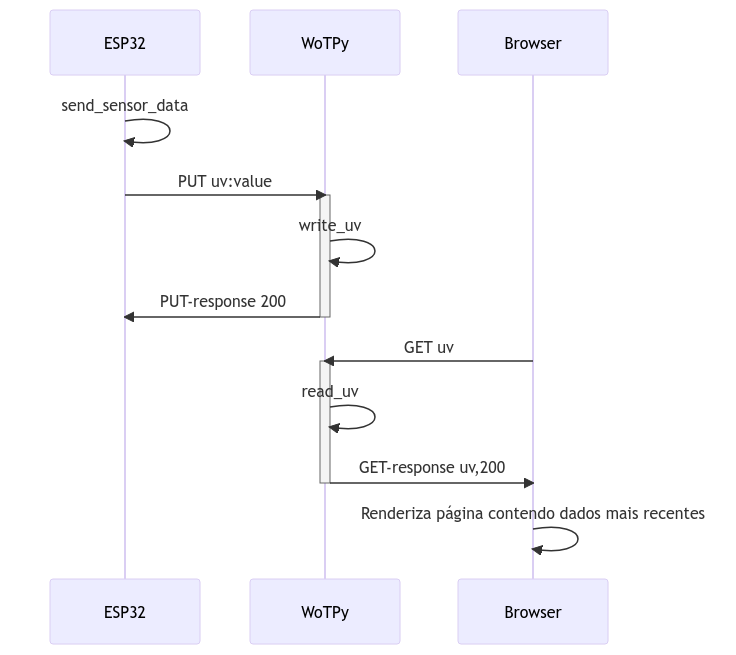
\includegraphics[scale=0.6]{figs/sequencia.png}
    \caption{O dispositivo (ESP32) executa um loop que, a cada 5 segundos executa a função send\_sensor\_data. Esta função envia uma requisição PUT para o servidor (WoTPy). Em resposta a essa requisição o servidor executa o handler (função) write\_uv que contém o envio da resposta. Um usuário pode acessar a informação no servidor através do Browser. Entrar a URL na barra de endereços do Browser o faz enviar ao servidor uma requisição GET. Em resposta à requisição o servidor executa o handler (função) read\_uv, que contém o envio da resposta - no caso, o valor de uv mais recente. O Browser recebe essa informação e renderiza a página contendo a informação.}
    \label{fig:sequencia}
\end{figure}


\chapter{Discussão}

A seção de discussão tem como objetivo analisar e interpretar os resultados obtidos no trabalho, relacionando-os com a literatura existente e abordando os principais pontos e contribuições do estudo.

\section{Análise dos Resultados}

Os resultados obtidos demonstraram que o WoTPy é uma solução viável para a implementação de um \textit{gateway} IoT baseado no W3C-WoT. Através da seleção cuidadosa das bibliotecas e ferramentas adequadas, foi possível desenvolver um gateway que suporta os principais protocolos de comunicação, como HTTP. Isso permite a integração de dispositivos IoT de diferentes fabricantes e facilita a interoperabilidade entre eles.

A compreensão das especificações do W3C-WoT foi essencial para o desenvolvimento do WoTPy. O estudo detalhado das especificações, como as Descrição das Coisas, Binding Templates e a \textit{Scripting API}, permitiu a implementação correta e eficiente do \textit{gateway}, garantindo a conformidade com os padrões estabelecidos.

A resolução dos problemas de instalação do WoTPy também se mostrou crucial. A simplificação do processo de instalação e configuração contribuiu para a fácil adoção do \textit{gateway} em diferentes ambientes e sistemas operacionais. Além disso, os testes e validação realizados confirmaram a qualidade e a funcionalidade do WoTPy, fornecendo confiabilidade e confiança na sua utilização.

\section{Comparação com Trabalhos Relacionados}

Ao comparar o WoTPy com outros \textit{gateways} IoT existentes, podemos observar suas vantagens e contribuições específicas. O WoTPy destaca-se por sua conformidade com as especificações do W3C-WoT, o que garante a interoperabilidade e a padronização no contexto da Web das Coisas. Além disso, sua flexibilidade e suporte aos principais protocolos de comunicação o tornam uma opção atrativa para a integração de dispositivos IoT heterogêneos.

A documentação detalhada e os exemplos de uso desenvolvidos também são diferenciais importantes do WoTPy. Esses recursos facilitam a compreensão e a utilização do gateway por parte dos desenvolvedores e usuários, contribuindo para a disseminação e adoção do projeto.

\section{Limitações e Possíveis Melhorias}

Durante o desenvolvimento deste trabalho, uma limitação identificada foi a incapacidade de utilizar o WoTPy no MicroPython. O MicroPython é uma implementação leve e eficiente do Python projetada para rodar em dispositivos com recursos limitados, como microcontroladores. No entanto, devido a diferenças de recursos e suporte a bibliotecas, o WoTPy não é atualmente compatível com o MicroPython.

Uma possível melhoria para contornar essa limitação seria a adaptação do WoTPy para ser compatível com o MicroPython. Isso permitiria que o gateway fosse implantado em dispositivos com recursos restritos, ampliando seu alcance e possibilitando sua utilização em uma variedade maior de cenários IoT. Essa adaptação envolveria ajustes nas dependências e otimizações específicas para o ambiente do MicroPython.

Além disso, uma outra melhoria potencial seria explorar alternativas de implementação específicas para o MicroPython. Isso poderia envolver a criação de uma versão simplificada do WoTPy ou o desenvolvimento de um gateway específico para dispositivos MicroPython. Essas abordagens permitiriam um melhor aproveitamento dos recursos limitados do MicroPython, garantindo a compatibilidade e a eficiência do gateway em tais dispositivos.

Essas melhorias seriam importantes para ampliar o alcance do WoTPy e torná-lo mais acessível a um maior número de dispositivos IoT, incluindo aqueles baseados no MicroPython. Ao superar a limitação atual e fornecer suporte para o MicroPython, o WoTPy se tornaria uma solução mais abrangente e versátil para a integração de dispositivos IoT em diferentes plataformas e ambientes.

\section{Contribuições e Impacto}

O presente trabalho contribui para o avanço da interoperabilidade e integração de dispositivos IoT no contexto da Web das Coisas. O desenvolvimento e a implementação do WoTPy como um gateway baseado no W3C-WoT oferecem uma solução prática e padronizada para a comunicação entre dispositivos de diferentes fabricantes.

As contribuições deste trabalho são relevantes tanto para a academia quanto para a indústria. Os resultados obtidos podem servir como base para futuras pesquisas e desenvolvimentos na área de IoT. Além disso, o WoTPy pode ser utilizado por empresas e profissionais que buscam criar soluções IoT interoperáveis e eficientes.

\section{Considerações Finais}

Através da metodologia adotada e da análise dos resultados, foi possível constatar que o WoTPy é uma solução eficaz para a implementação de um gateway IoT baseado no W3C-WoT. Suas funcionalidades, conformidade com as especificações do W3C e facilidade de uso o tornam uma opção viável e promissora no contexto da Web das Coisas.

O trabalho realizado contribui para a disseminação e adoção do WoTPy, bem como para a melhoria da interoperabilidade e integração de dispositivos IoT. Espera-se que as limitações identificadas possam ser superadas e que as melhorias sugeridas possam ser implementadas em trabalhos futuros.

\chapter{Conclusão}

A integração do WoTPy com grafos de conhecimento na Internet das Coisas (IoT) representa uma evolução significativa na análise de dados, na interoperabilidade entre dispositivos e na personalização e contextualização de soluções IoT. Esta integração abre novas possibilidades para aplicações mais inteligentes e eficientes, ao mesmo tempo em que impulsiona inovações e contribui para o desenvolvimento de padrões e protocolos em IoT.

Um dos principais avanços proporcionados por esta integração é o enriquecimento da análise de dados. Ao utilizar grafos de conhecimento, os dados coletados de dispositivos IoT podem ser interpretados não apenas em termos quantitativos, mas também qualitativos. Isso oferece uma compreensão mais profunda e contextualizada dos dados, permitindo aplicações que podem responder de maneira mais precisa e eficiente a condições variáveis. Tal capacidade de análise enriquecida abre caminho para soluções IoT que são mais inteligentes e adaptáveis às necessidades específicas dos usuários.

Outro avanço significativo é a facilitação da interoperabilidade em IoT. Tradicionalmente, um dos maiores desafios em IoT é a interoperabilidade entre dispositivos de diferentes fabricantes e plataformas. A integração do WoTPy com grafos de conhecimento aborda eficientemente esse desafio, promovendo uma comunicação mais fluida e eficaz entre dispositivos heterogêneos. Isso simplifica não apenas o desenvolvimento de sistemas IoT, mas também melhora a experiência do usuário final.

Além disso, a integração impulsiona a personalização e contextualização em IoT. As soluções desenvolvidas podem ser profundamente personalizadas e contextualizadas para as necessidades específicas dos usuários, graças à análise semântica profunda proporcionada pelos grafos de conhecimento. Essa capacidade de adaptar-se ao contexto específico de uso é crucial para aplicações que exigem um alto grau de personalização.

Esta integração também abre portas para novas aplicações IoT, especialmente em áreas que exigem análises complexas e adaptação a contextos dinâmicos. Cidades inteligentes, saúde digital, agricultura inteligente e automação residencial são apenas alguns exemplos de áreas que podem se beneficiar imensamente dessa integração. A capacidade de analisar dados IoT em um nível semântico também fomenta inovações em inteligência artificial e aprendizado de máquina, onde a interpretação contextualizada dos dados é essencial.

Adicionalmente, a integração pode levar a um aumento da eficiência e redução de custos em sistemas IoT. Melhorar a interoperabilidade e fornecer análises mais profundas pode resultar em sistemas mais eficientes, reduzindo os custos operacionais e de manutenção e melhorando a eficiência energética dos dispositivos.

Por fim, a integração contribui para a evolução dos padrões e protocolos em IoT, sugerindo um modelo para a incorporação de tecnologias de dados semânticos em sistemas IoT existentes e futuros. Contudo, também traz desafios, como a gestão eficaz dos grafos de conhecimento em grande escala e a garantia de segurança e privacidade dos dados, que são campos importantes para pesquisas e desenvolvimentos futuros.

% ----------------------------------------------------------
% ELEMENTOS PÓS-TEXTUAIS
% ----------------------------------------------------------
\postextual
% ----------------------------------------------------------

% ----------------------------------------------------------
% Referências bibliográficas
% ----------------------------------------------------------
\bibliography{referencias}

%---------------------------------------------------------------------
% INDICE REMISSIVO
%---------------------------------------------------------------------
%%%%%MF\phantompart
%%%%%MF\printindex
%---------------------------------------------------------------------

\end{document}
